%!TEX TS-program = xelatex
%!TEX encoding = UTF-8 Unicode

\documentclass[12pt]{extarticle}
% extarticle is like article but can handle 8pt, 9pt, 10pt, 11pt, 12pt, 14pt, 17pt, and 20pt text

\def \ititle {Origins of Mind}
 
\def \isubtitle {Lecture 01}
 
\def \iauthor {Stephen A. Butterfill}
\def \iemail{s.butterfill@warwick.ac.uk}
\date{}

%for strikethrough
\usepackage[normalem]{ulem}

\input{$HOME/Documents/submissions/preamble_steve_handout}

%\bibpunct{}{}{,}{s}{}{,}  %use superscript TICS style bib
%remove hanging indent for TICS style bib
%TODO doesnt work
\setlength{\bibhang}{0em}
%\setlength{\bibsep}{0.5em}


%itemize bullet should be dash
\renewcommand{\labelitemi}{$-$}

\begin{document}

\begin{multicols}{3}

\setlength\footnotesep{1em}


\bibliographystyle{newapa} %apalike

%\maketitle
%\tableofcontents




%--------------- 
%--- start paste


\def \ititle {Origins of Mind}
 
\def \isubtitle {Lecture 01}
 
 
 
\
 
 
 
\begin{center}
 
{\Large
 
\textbf{\ititle}: \isubtitle
 
}
 
 
 
\iemail %
 
\end{center}
 
 
 
\section{The Question}
 
‘... ’tis past doubt, that Men have in their Minds several Ideas, such as are those expressed by the words, Whiteness, Hardness, ... and others: It is in the first place to be enquired, How he comes by them?’
\citep[p.\ 104]{Locke:1975qo}
 
‘How does it come about that the development of organic behavior into controlled inquiry brings about the differentiation and cooperation of observational and conceptual operations?’
\citep[p.\ 12]{Dewey:1938yp}
 
‘the fundamental explicandum, is the organism and its propositional attitudes ... Cognitive psychologists accept ... the ... necessity of explaining how organisms come to have the attitudes to propositions that they do.’
\citep[p.\ 198]{Fodor:1975pb}
 
\textbf{Question}
How do humans come to know about---and to knowingly manipulate---objects, causes, words, numbers, colours, actions and minds?
 
 
 
\section{From Myths to Mechanisms}
 
‘the soul inherently contains the sources of various notions and doctrines which external objects merely rouse up on suitable occasions’
\citep[p.\ 48]{Leibniz:1996bl}
 
‘Men, barely by the Use of their natural Faculties, may attain to all the Knowledge they have, without the help of any innate Impressions; [...]
‘it would be impertinent to suppose, the Ideas of Colours innate in a Creature, to whom God hath given Sight, and a Power to receive them by the Eyes from external Objects’
\citep[p.\ 48]{Locke:1975qo}
 
‘Developmental science [...] has shown that both these views are false’
\citep[p.\ 89]{Spelke:2007hb}.
 
 
 
\section{Inbetween mindless behaviour and thought}
 
‘We have many vocabularies for describing nature when we regard it as mindless, and we have a mentalistic vocabulary for describing thought and intentional action; what we lack is a way of describing what is in between’ \citep[p.\ 11]{Davidson:1999ju}
 
\textit{Object permanence}:
the ability to know things about, or represent, objects you aren't currently perceiving.
 
\begin{center}
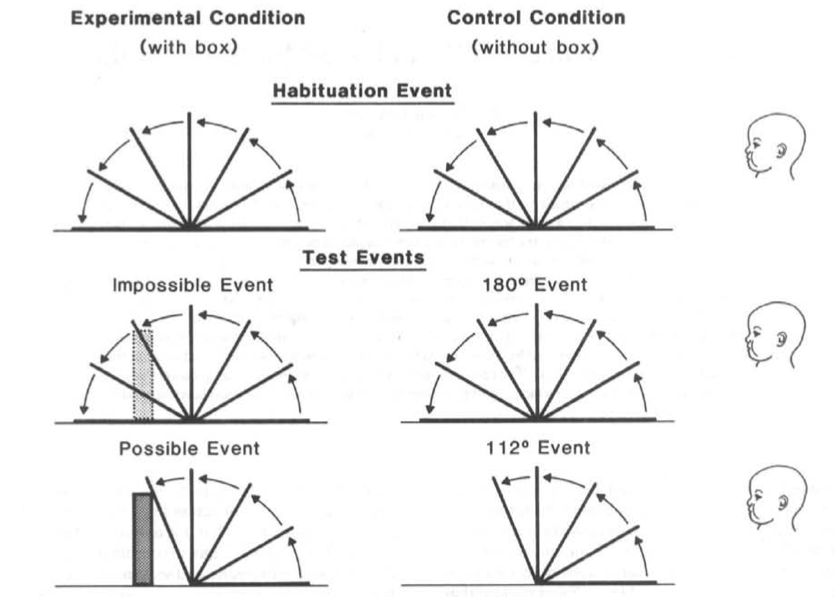
\includegraphics[scale=0.3]{../www.slides/src/files/img/baillargeon_1987_fig1.neg.png}
\end{center}
\begin{center} \citealp{baillargeon:1987_object} figure 1 \end{center}
 
\begin{center}
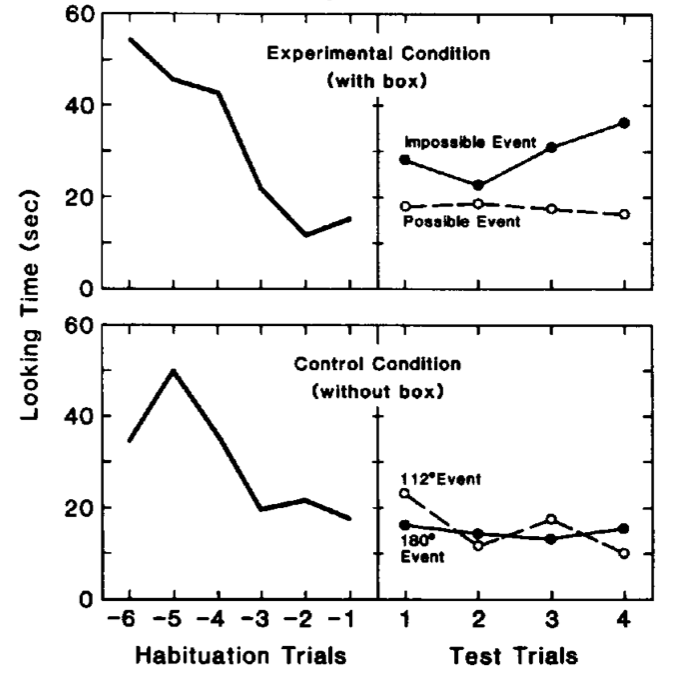
\includegraphics[scale=0.3]{../www.slides/src/files/img/baillargeon_1987_fig2.neg.png}
\end{center}
\begin{center} \citealp{baillargeon:1987_object} figure 2 \end{center}
 
‘there are many separable systems of mental representations ... and thus many different kinds of knowledge. ... the task ... is to contribute to the enterprise of finding the distinct systems of mental representation and to understand their development and integration’
\citep[p.\ 1522]{Hood:2000bf}.
 
‘violation-of-expectation experiments, using looking-time measures, suggested that infants have object permanence in occlusion conditions; but simplified-search studies confirm that infants fail to reach towards occluded objects, suggesting that infants do not have object permanence in occlusion conditions. This discrepancy, however, is only the tip of the iceberg. Results of studies attempting to measure infants’ cognitive abilities using reaching measures often contradict results gained while using looking-time measures.’ \citep[p.\ 994]{charles:2009_object}
 
\subsection{Dennett’s Intentional Stance}
 
(a) \textit{The strategy} ‘Here is how it works: first you decide to treat the object whose behavior is to be predicted as a rational agent; then you figure out what beliefs that agent ought to have, given its place in the world and its purpose. Then you figure out what desires it ought to have, on the same considerations, and finally your predict that this rational agent will act to further its goals in the light of its beliefs. A little practical reasoning from the chosen set of beliefs and desires will in many---but not in all---instances yield a decision about what the agent ought to do; that is what you predict the agent will do.’
\citep[p.\ 17]{Dennett:1987sf}
 
(b) \textit{The metaphysics} ‘any object---or as I shall say, any system---whose behavior is well predicted by this strategy is in the fullest sense of the word a believer. What it is to be a true believer is to be an intentional system, a system whose behavior is reliably and voluminously predictable via the intentional strategy.’
\citep[p.\ 15]{Dennett:1987sf}
 
 
 
\section{Social Interaction}
 
\subsection{A Conjecture}
 
‘humans acquire knowledge at a pace far outstripping that found in any other species. Recent evidence indicates that interpersonal understanding—in particular, skill at inferring others’ intentions—plays a pivotal role in this achievement.’
\citep[p.\ 40]{Baldwin:2000qq}
 
‘functions traditionally considered hallmarks of individual cognition originated through the need to interact with others ...\ perception, action, and cognition are grounded in social interaction.’
\citep[p.\ 103]{Knoblich:2006bn}
 
Vygotskian Intelligence Hypothesis:
‘the unique aspects of human cognition ... were driven by, or even constituted by, social co-operation.’
\citep[p.\ 1]{Moll:2007gu}
 
‘human cognitive abilities ... [are] built upon social interaction’
\citep{sinigaglia:2008_roots} %*page
 
\subsection{How do children acquire words?}
 
‘children learn words through the exercise of reason’
(\citealp[p.\ 1103]{Bloom:2001ka}; see \citealp{Bloom:2000qz})
 
‘Augustine describes the learning of human language as if the child came into a strange country and did not understand the language of the country; that is, as if it already had a language, only not this one. Or again: as if the child could already think, only not yet speak.’
\citep[15--16, §32]{Wittgenstein:1953mm}
 
‘[t]he child learns this language from the grown-ups by being trained to its use. I am using the word ‘trained’ in a way strictly analogous to that in which we talk of an animal being trained to do certain things. It is done by means of example, reward, punishment, and suchlike’
\citep[p.\ 77]{Wittgenstein:1972lj}
 
‘the child's early learning of a verbal response depends on society's reinforcement of the response in association with the stimulations that merit the response’
(\citep[p.\ 82]{Quine:1960fe}; compare \citep[pp.\ 28--9]{Quine:1974rd})
 
‘A child learning to speak is learning habits and associations which are just as much determined by the environment as the habit of expecting dogs to bark and cocks to crow’
\citep[p.\ 71]{Russell:1921ww}
 
Children acquiring language create their own words before they learn to use those of the adults around them.
 
‘Some children are so impatient that they coin their own demonstrative pronoun. For instance, at the age of about 12 months, Max would point to different objects and say “doh?,” some¬times with the intent that we do something with the objects, such as bring them to him, and sometimes just wanting us to appreciate their existence’
(\citealp[p.\ 122]{Bloom:2000qz}; see further \citealp{Clark:1981bi,Clark:1982hj}).
 
Even where children have mastered a lexical convention, they will readily violate it in their own utterances in order to get a point across.
 
‘From the time they first use words until they are about two or two-and-a-half, children noticeably and systematically overextend words. For example, one child used the word “apple” to refer to balls of soap, a rubber-ball, a ball-lamp, a tomato, cherries, peaches, strawberries, an orange, a pear, an onion, and round biscuits’
\citep[p.\ 35]{Clark:1993bv}
 
Children with no experience of others' languages can create their own languages.
\citep{Kegl:1999es,Senghas:2001zm,Goldin-Meadow:2003pj}
 
 
 
\section{Core knowledge}
 
Interpreting violation-of-expectation experiments:
 
‘evidence that infants look reliably longer at the unexpected than at the expected event is taken to indicate that they (1) possess the expectation under investigation; (2) detect the violation in the unexpected event; and (3) are surprised by this violation. The term surprise is used here simply as a short-hand descriptor, to denote a state of heightened attention or interest caused by an expectation violation.’
\citep[p.\ 168]{wang:2004_young}
 
\subsection{Principles of Object Perception \citep{Spelke:1990jn}}
 
cohesion—‘two surface points lie on the same object only if the points are linked by a path of connected surface points’
 
boundedness—‘two surface points lie on distinct objects only if no path of connected surface points links them’
 
rigidity—‘objects are interpreted as moving rigidly if such an interpretation exists’
 
no action at a distance—‘separated objects are interpreted as moving independently of one another if such an interpretation exists’
 
 

%--- end paste
%--------------- 
 
\footnotesize 
\bibliography{$HOME/endnote/phd_biblio}

\end{multicols}

\end{document}